% Testes
% 	-Intro
% 	-Teste da Localização
% 		Fazer medidas da distância real do aparelho do kinect e comparar com a medida dada pelo kinect, montar um gráfico ou algo que mostre o erro.
% 	-Teste do Reconhecimento
% 		Fazer uma matriz de confusão.
% 	-Teste do Rastreamento
% 		Testar a detecção e o rastreamento, falar do problema com obstrução
% 	-Teste da Integração
% 		Falar do UserApp desenvolvido para testar o driver
\chapter{Resultados e Análises}

% \section{\textit{SmartSpace} Laico}

% 	O ambiente para o qual o sistema \textit{True} será projetado, desenvolvido e testado chama-se LAICO (\textbf{LA}boratório de sistemas \textbf{I}ntegrados e \textbf{CO}ncorrente), um laboratório do Departamento de Ciência da Computação da Universidade de Brasília. O LAICO possui dimensões de, aproximadamente,  $\displaystyle 7,67m$ x $\displaystyle 6,45m$ ilustrado pela Figura~\ref{fig:laico}.

% 	\begin{figure}[hbt]
% 			\begin{center}
% 				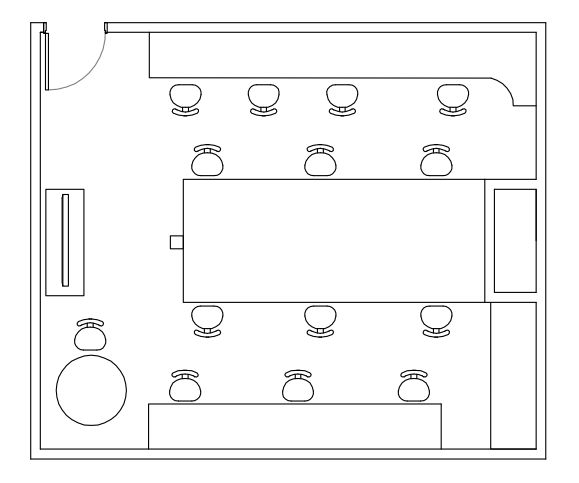
\includegraphics[scale=0.6]{figuras/4.ProblemaEProposta/laico.png}
% 			\end{center}
% 			\caption{Planta do \textit{SmartSpace} Laico.}
% 			\label{fig:laico}
% 		\end{figure}	

\section{Rastreamento dos Usuários}

\section{Localização dos Usuários}

\section{Identificação dos Usuários}

\section{Integração com middleware \textit{UbiquitOS}}

	Com intuito de exemplificar a utilização do \textit{UserDriver} e testar a integração do Sistema TRUE com o middleware \textit{UbiquitOS} foi desenvolvido uma aplicação para o middleware chamada \textit{UserApp} cujo diagrama de classe é mostrado na Figura~\ref{fig:diagrama-userapp}. Esta aplicação registra um \textit{listener} para ``escutar'' os eventos do \textit{UserDriver} chamado \textit{UserListener}. A Figura~\ref{fig:diagrama-userlistener} mostra o diagrama de classe do \textit{UserListener}.

		\begin{figure}[hbt]
			\begin{center}
				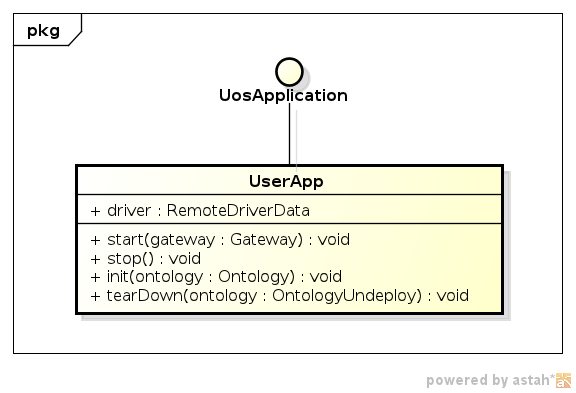
\includegraphics[scale=0.6]{figuras/5.Testes/diagrama-classe-user-ap.png}
			\end{center}
			\caption{Diagrama de Classe da aplicação \textit{UserApp}.}
			\label{fig:diagrama-userapp}
		\end{figure}

		\begin{figure}[hbt]
			\begin{center}
				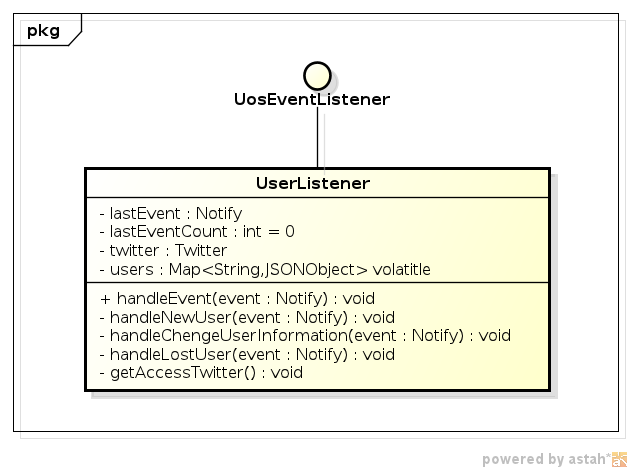
\includegraphics[scale=0.6]{figuras/5.Testes/diagrama-classe-user-listener.png}
			\end{center}
			\caption{Diagrama de Classe do \textit{listener} \textit{UserListener}.}
			\label{fig:diagrama-userlistener}
		\end{figure}

	Basicamente, quando o \textit{UserListener} obtém os eventos do \textit{UserDriver} envia mensagens pelo Twitter para os usuários no ambiente, conforme o evento recebido. A Figura~\ref{fig:diagrama-tweet} mostra o fluxo básico de execução do \textit{listener} e as mensagens padrões para cada tipo de evento recebido. Para enviar as mensagens pelo Twitter foi utilizado a biblioteca \textit{twitter4j}. 

	\begin{figure}[hbt]
			\begin{center}
				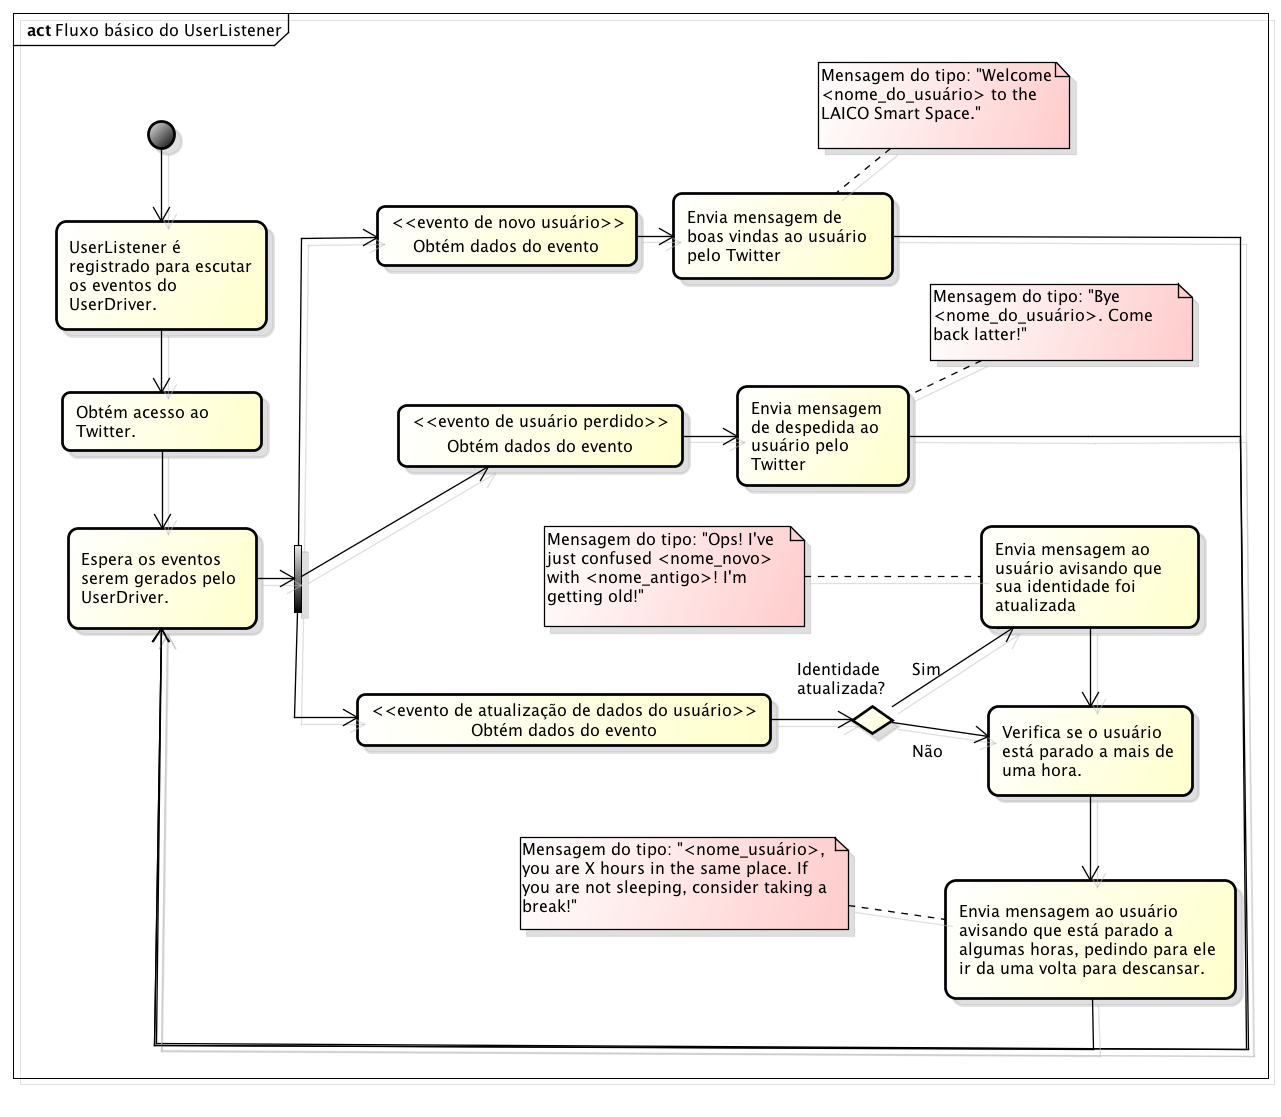
\includegraphics[scale=0.45]{figuras/5.Testes/diagrama-user-tweet.png}
			\end{center}
			\caption{Fluxo básico de execução do \textit{listener} \textit{UserListener}.}
			\label{fig:diagrama-tweet}
		\end{figure}












